\section{Preparacion del equipo}

\subsection{Respaldo de datos}

Mi equipo cuenta con dos espacios de almacenamiento un SSD de 258GB en el que tiene instalado el sistema operativo windows y un disco duro de 1TB, en este se instalara el sistema linux para ello realicé una revision de la informacion que contenia para ver si era relevante respaldarla o no la mayor parte de la informacion fue eliminada. 

Una vez revisada toda la información y seleccionada la que queria preservar en un disco duro externo relice la copia de los datos.

\subsection{Descarga de los prerequisitos}

\subsubsection{Instalación de la iso}
Nos dirgimos a la pagina de \href{https://pop.system76.com/}{Pop OS} y seleccionamos la iso que nos interese, en mi caso seleccioné la iso que viene con los drivers de NVIDIA pre-instalados.

\begin{figure}[h]
  \begin{center}
    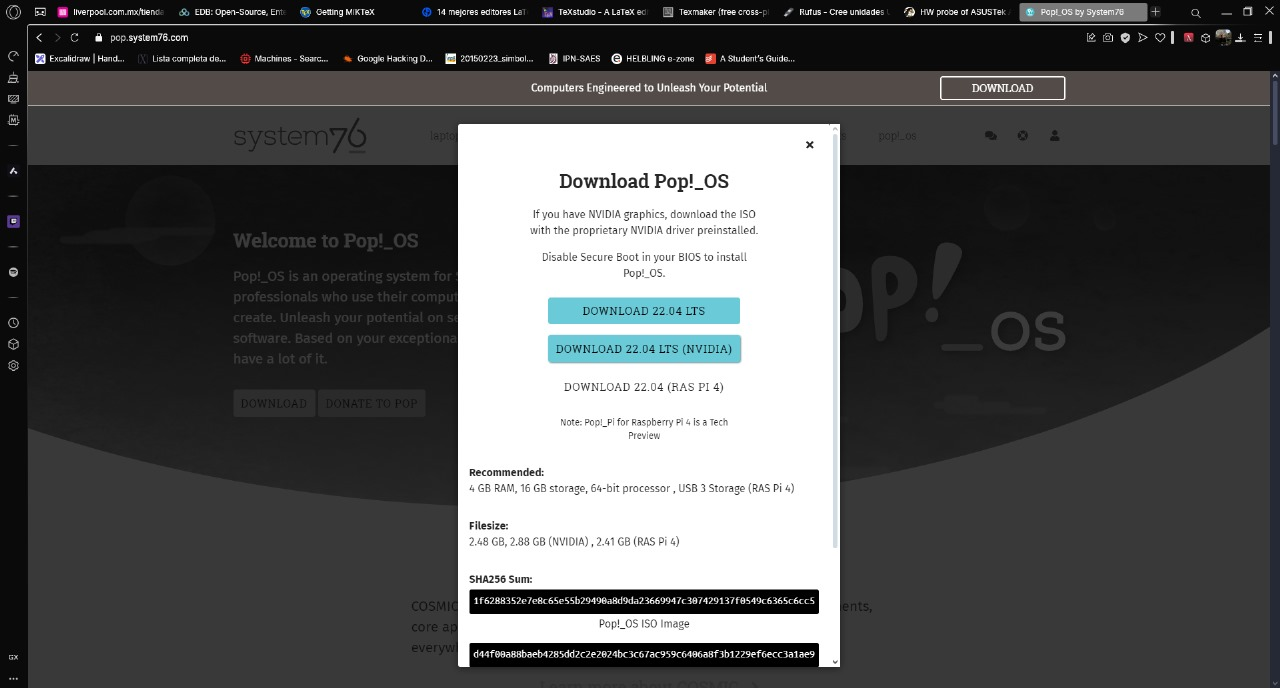
\includegraphics[width=0.95\textwidth]{img/download_popos.jpeg}
  \end{center}
  \caption{Descarga de la iso con drivers NVIDIA}\label{fig:download_popos}
\end{figure}

\clearpage
\subsubsection{Instalación de Rufus}

Una vez teniendo la iso procedemos a la instalacion de un programa para flashear una USB, para ello nos dirigimos a la pagina oficial de nuestro flasher \href{https://rufus.ie/es/}{Rufus} y descargamos el ejecutable.

Yo descaargue la versión portable para mayor comodidad. 

\begin{figure}[h]
  \begin{center}
    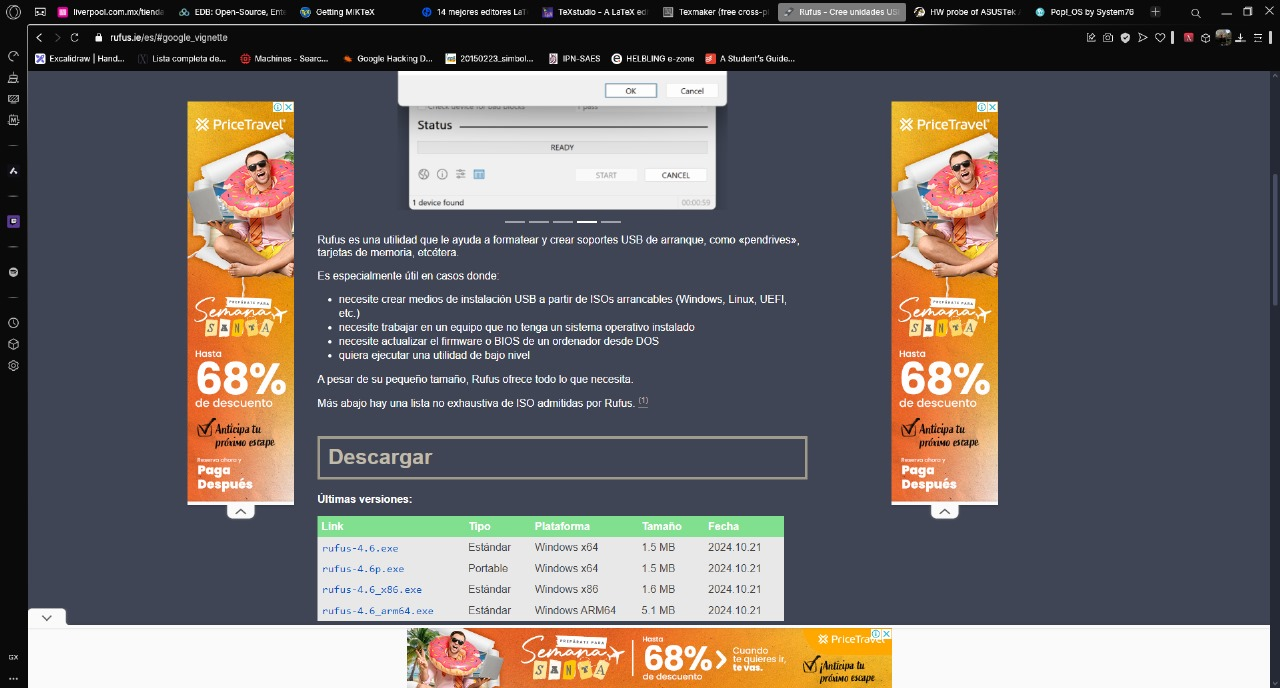
\includegraphics[width=0.75\textwidth]{img/download_rufus.jpeg}
  \end{center}
  \caption{Descarga de Rufus}\label{fig:download_rufus}
\end{figure}


\subsection{Flasheo de la USB}

Con la iso descargada y rufus listo procedemos a conectar la usb que usaremos para instalar nuestro sistema operativo.
\\\\
A continuación los pasos que seguí para la instalación
\begin{enumerate}
  \item Abrimos Rufus
  \item Seleccionamos la iso
  \item Seleccionamos el tipo de boot (UEFI/BIOS)
  \item Seleccionamos la USB
  \item Formateamos la USB y comienza la descompresion de la iso
\end{enumerate}

\begin{figure}[h]
  \begin{center}
    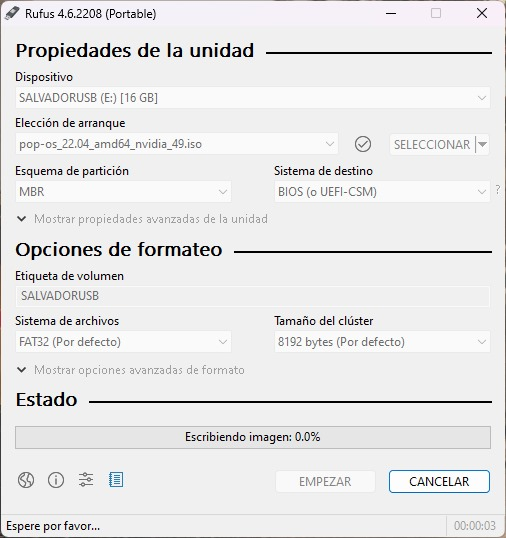
\includegraphics[width=0.3\textwidth]{img/usb_boot.jpeg}
  \end{center}
  \caption{Flasheo de USB}\label{fig:usb_boot}
\end{figure}

\\
Y esperamos que la instalacion finalice, esto puede llevar desde un par de minutos hasta una hora dependiendo del tamaño del sistema operativo.


\subsection{Instalación del sistema en el disco}

Con todo preparado podemos apagar la computadora y encenderla para entrar en el menú de arranque, en mi computadora se utiliza la tecla \keys{F2}; una vez en el menú se selecciona la USB booteable como método de arranque. 
\\
Con esto realizado se abrira la pantalla principal del sistema operativo(Vease \autoref{fig:pop_os_desktop})

\begin{figure}[h]
  \begin{center}
    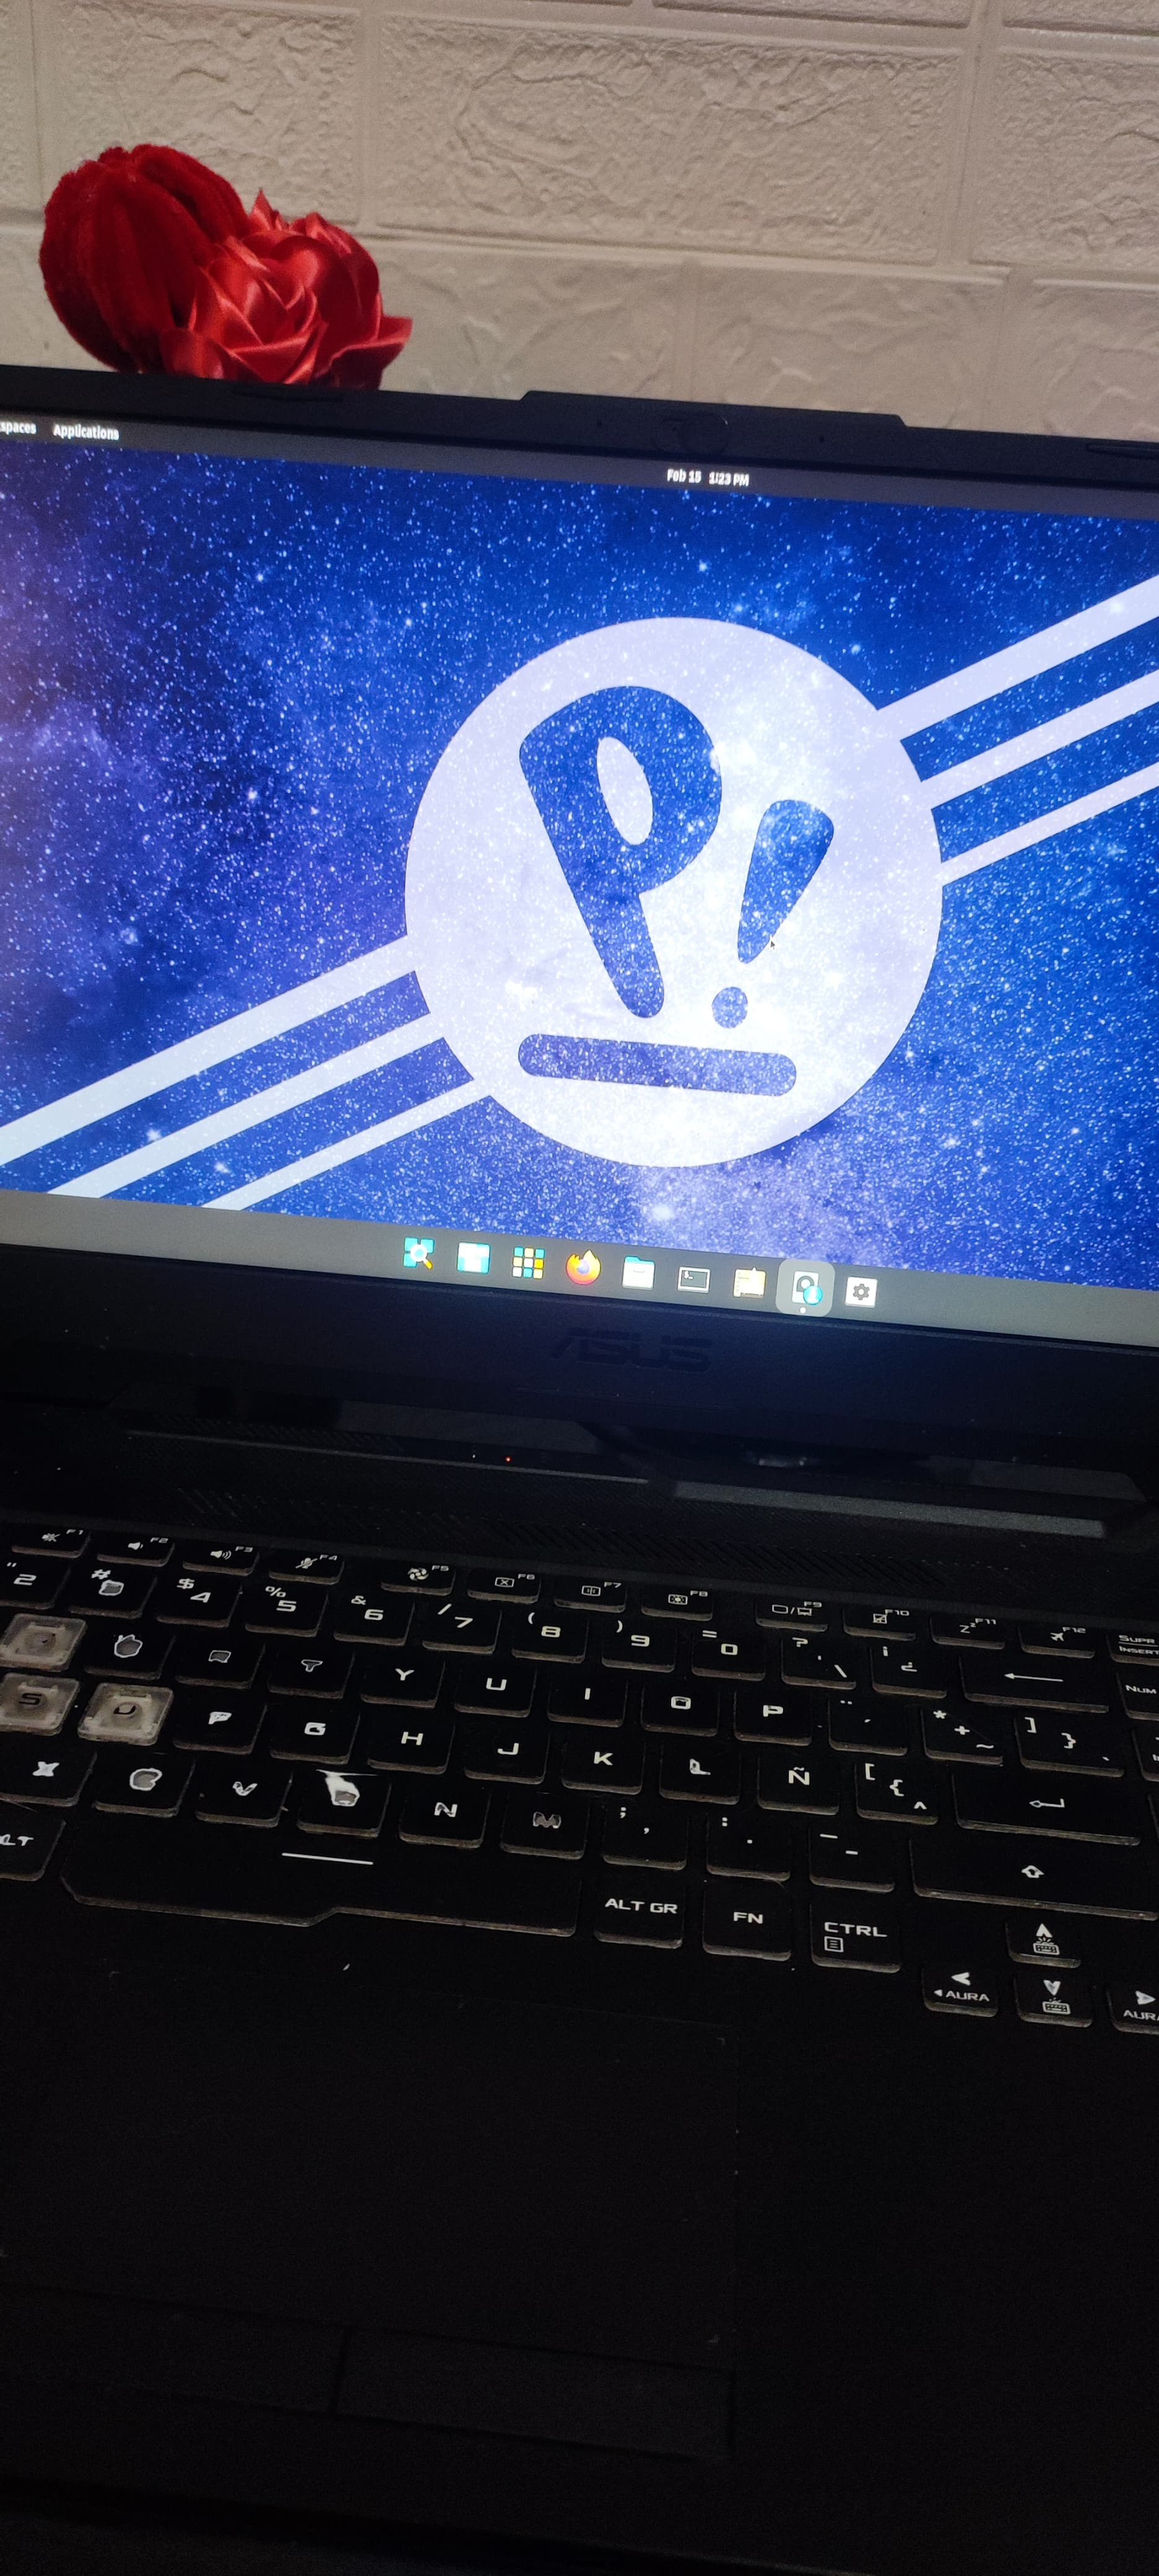
\includegraphics[width=0.25\textwidth]{img/pop_os_desktop.jpeg}
  \end{center}
  \caption{Escritorio de Pop OS}\label{fig:pop_os_desktop}
\end{figure}

Abrimos la aplicación de encargada de la instalación, seleccionamoos el idioma de la instalación y la distribucion de teclado apropiada. 
Una vez hecho esto procedemos a crear las particiones del sistema.

\begin{table}[h]
  \centering
  \begin{tabular}{ |p{3cm}|p{3cm}|p{3cm}|  }
    \hline
    \multicolumn{3}{|c|}{Configuración de particiones} \\
    \hline
    Partición & Tamaño & Sistema de archivos\\
    \hline
    EFI & 2.1 GB & FAT-32\\
    SWAP & 17GB & SWAP\\
    ROOT & 981GB & EXT4\\
    \hline
  \end{tabular}
  \label{tab:particiones}
  \caption{Tabla de particiones}
\end{table}

Dejamos que se limpie y se formateé el disco duro. 

\begin{figure}[h]
  \begin{center}
    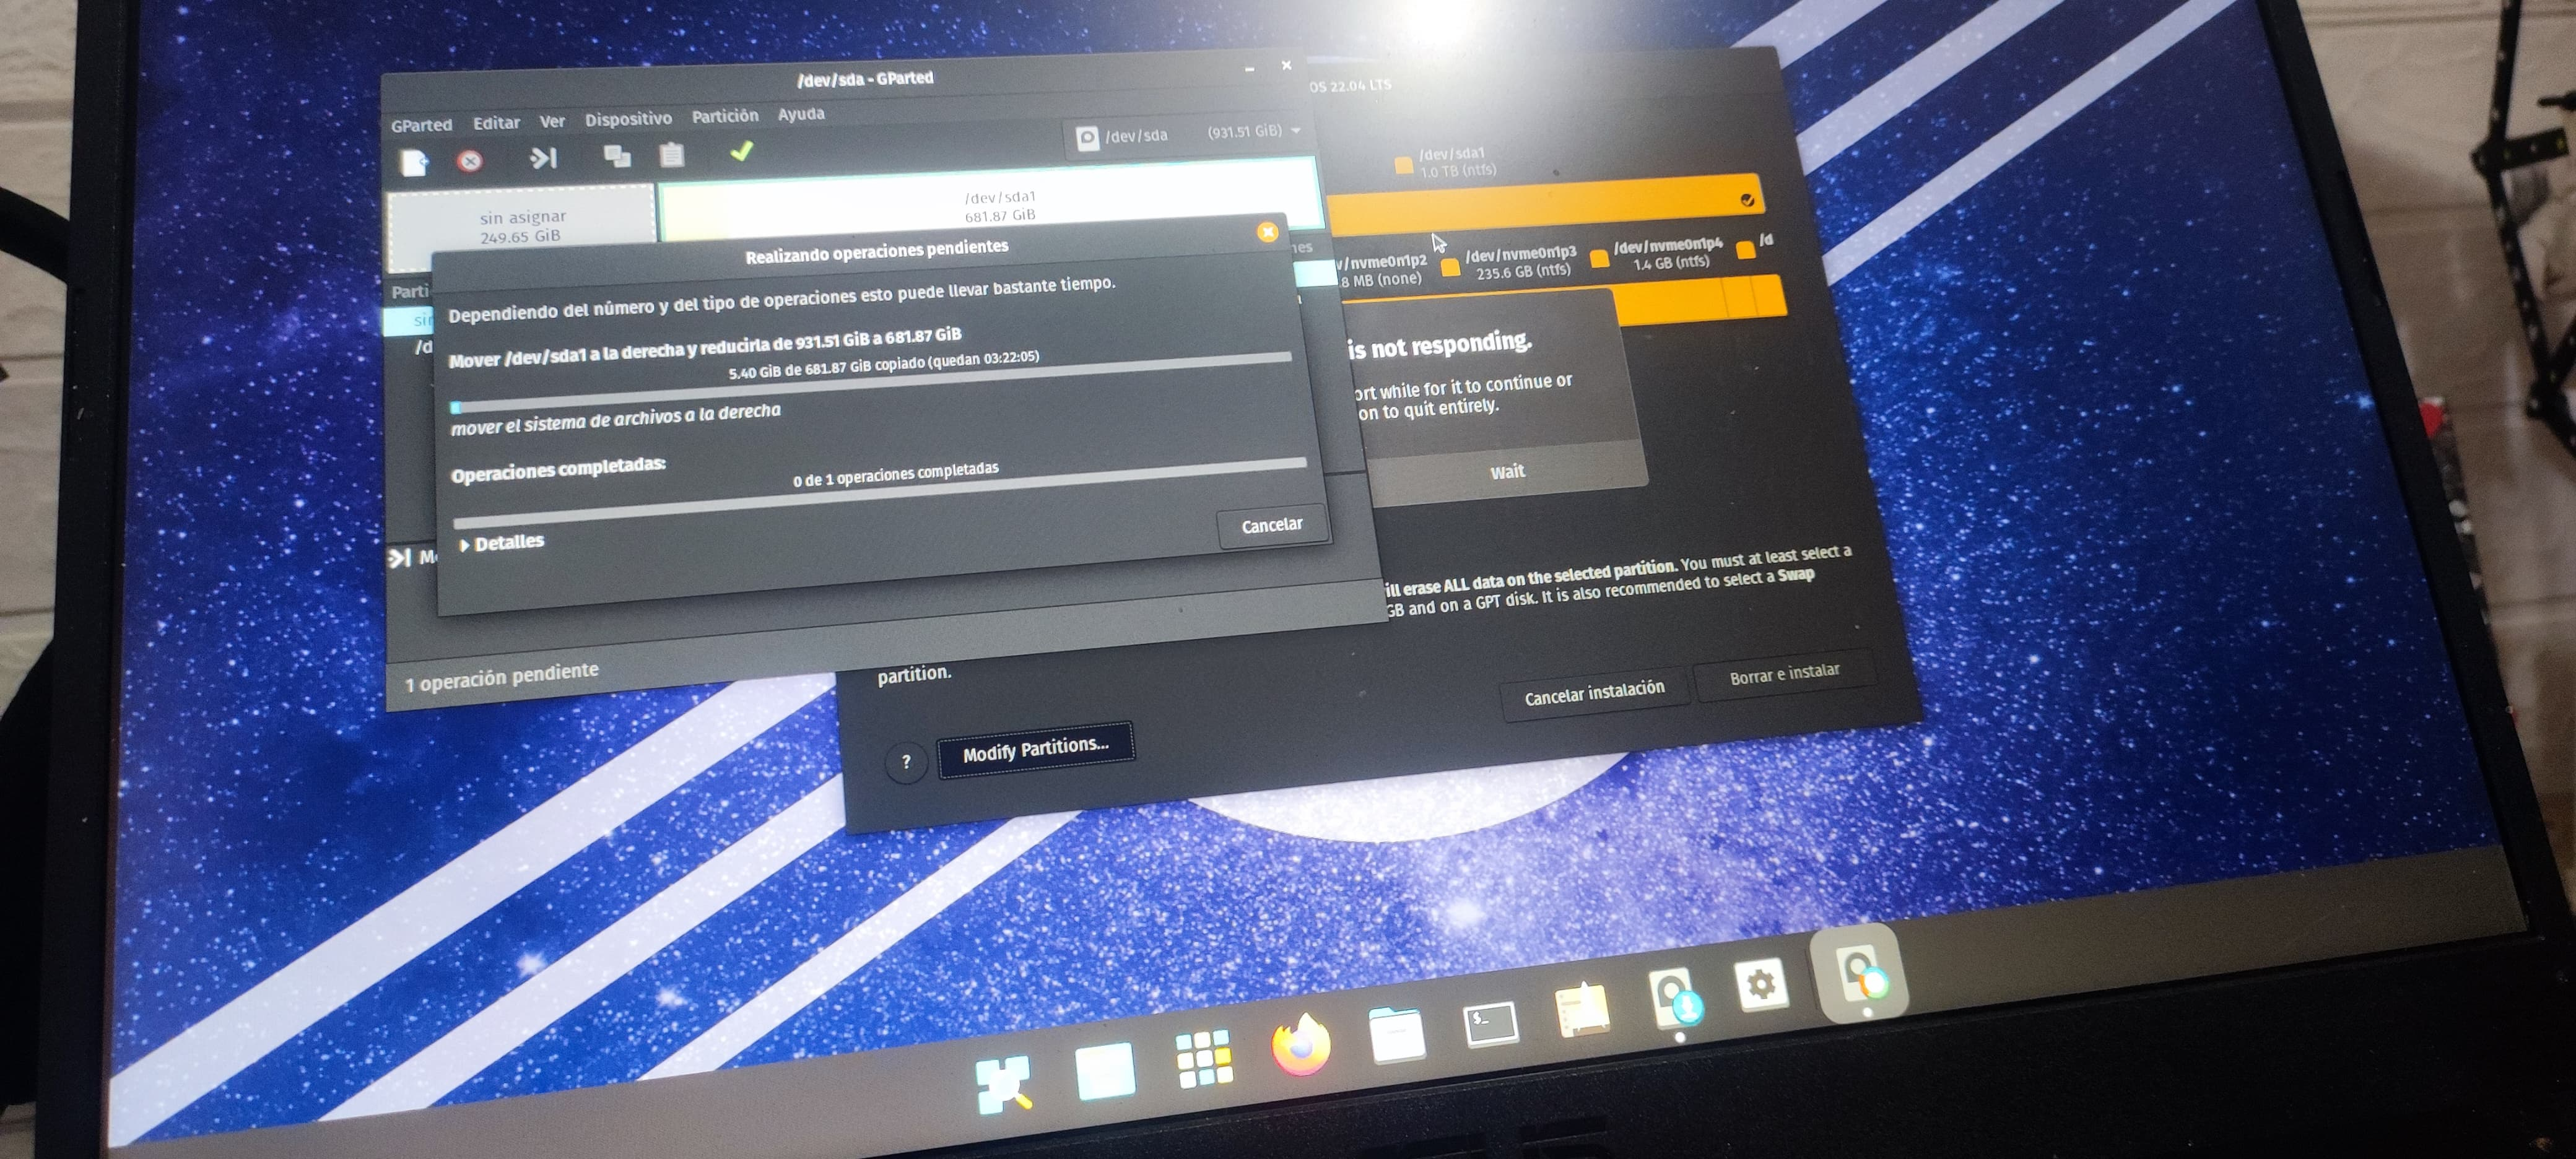
\includegraphics[width=0.3\textwidth]{img/particionado.jpeg}
  \end{center}
  \caption{Creando las particiones}\label{fig:particionado}
\end{figure}


Una ves formateado te pedira la creacion de un usuario y contraseña procedes con la instalacion y reinicias la computadora, cuando este reiniciando puedes quitar la usb y se iniciara directamente en el sistema operativo recien instalado. 

Inicias la sesión con el usuario que creaste anteriormente abres la terminal y aactualizas el sistema con los siguientes comandos:

\begin{lstlisting}[language=Bash]
  sudo apt update
  sudo apt upgrade
\end{lstlisting}

